\documentclass[11pt,a4paper]{article}
\usepackage[margin=2.4cm]{geometry}
\usepackage{amsmath,amssymb,amsfonts}
\usepackage{booktabs}
\usepackage{graphicx}
\usepackage[dvipsnames]{xcolor}
\usepackage{hyperref}
\usepackage{booktabs}
\usepackage{caption}
\captionsetup{font=small,labelfont=bf}

\title{Beyond Optimistic Planning: When Does Learning Stochastic User Dynamics\\
Make Recommendation Planning Better?}
\author{Arina Romashkina\\
\small AI VK / Scientific Studio research project\\
\small \url{github.com/arinaromashkina/planning_over_MF_MDP}}
\date{November 2026}

\newcommand{\J}{J(\pi)}
\newcommand{\E}{\mathbb{E}}

\begin{document}
\maketitle

\begin{abstract}
The MF-MDP formulation casts top-K retrieval as planning over the implicit-ALS
posterior: the state is the fold-in posterior $(P,u)$, the transition is a closed-form
rank-one update that \emph{optimistically} assumes every recommendation is accepted, and
the reward mixes cosine relevance with a posterior-alignment term. We reproduce this
method and show that, on MovieLens-1M under the leave-last-$n$ protocol, the static
baseline is reproduced (Recall@10 0.0704 vs.\ 0.0694 reported) but the reported planning
gains are not. A leverage analysis explains why: the quantity driving the reward's
alignment term is bounded by $\approx d/n_{\text{items}}$ for spread embedding
geometries and correlates with item popularity rather than user relevance, leaving the
planning layer quality-inert. We then ask whether \emph{learning stochastic user
responses} fixes this. In two controlled environments with known generative dynamics and
exact oracles we show that feedback-conditioned stochastic planning reaches the oracle
and beats the optimistic planner by $+0.122$ (paired bootstrap CI95 $[0.115, 0.129]$)
when the state representation is faithful, and does not differ from it ($-0.004$, CI95
$[-0.010, 0.002]$) when the state is a compressed MF posterior. The benefit of deeper
planning is governed by the same bottleneck: regret falls $5$--$15\times$ from depth-2 to
full-horizon planning once the model is reasonable, and response-model estimation error
stops being binding once the model saturates. On KuaiRand-1K, graded engagement
(watch-ratio) is predictable and transfers to randomized exposure (AUC $0.839 \to
0.826$), while binary click prediction is policy-bound and temporally miscalibrated
(ECE $0.234$). Our answer to ``when does learning a stochastic recommendation environment
make planning better?'' is: only when the state representation carries the dynamics ---
otherwise the transition model's sophistication is irrelevant.
\end{abstract}

\section{Introduction}

A recommendation is never an isolated event. A consumed item changes the user, and
therefore what should be retrieved next; a poor pick can end the session or push the
user into an irrelevant region of the catalog. Sequential recommendation is naturally a
Markov decision process: the state describes the user's current context, the action is
the recommended item, the reward is the user's feedback, and the transition encodes how
the state evolves. Exploiting this structure for \emph{candidate generation} --- quickly
selecting a small set of promising items from a large catalog --- is the goal of the
starting paper~\cite{trapeznikov2026mfmdp}, which builds an MDP directly on the
implicit-ALS posterior. The user state is the pair $(P, u)$ where $P = A^{-1}$ is the
inverse precision of the fold-in least-squares problem, actions are catalog items with
fixed embeddings, and the transition is a closed-form Sherman--Morrison rank-one
update~\cite{sherman1950morrison} that folds the recommended item in as \emph{accepted}
positive feedback --- an \textbf{optimistic} dynamics model. The reward combines a
cosine relevance term with a posterior-alignment term driven by the leverage
$\ell = v^{\top} P v$, and the compared planners span static retrieval, one-step
lookahead (Plan-1), and horizon-$K$ MCTS (Plan-K).

The optimistic transition is, however, a misspecified model of the user: real users
skip, partially consume, dislike, or leave. Whether planning over such a posterior helps
at all --- and whether replacing the optimistic assumption with a \emph{learned
stochastic response model} changes the answer --- is an open and falsifiable question.
It cannot be answered from logged-data metrics alone, because the counterfactual
dynamics are unobservable: responses to unexposed items are unknown, and the logging
policy confounds what is visible.

\paragraph{What exists.}
Learned world models for recommendation are an active area. MCRL~\cite{li2023mcrl}
learns reward and transition structure with contrastive objectives; ROLeR~\cite{zhang2024roler}
and R3S~\cite{shu2025r3s} refine reward models and uncertainty penalties; KuaiSim~\cite{zhao2023kuaisim},
RecSim NG~\cite{hsu2021recsimng}, and the KuaiEnv of CIRS~\cite{gao2023cirs} provide
hand-built simulators; a recent session-level REINFORCE method~\cite{matveev2026sessionreinforce}
simulates user feedback at test time; WMG-RL~\cite{li2026wmg} distills a frozen user
engagement world model into a policy. Model-based RL contributes the planning machinery:
MuZero~\cite{schrittwieser2020muzero}, Sampled MuZero~\cite{hubert2021sampledmuzero} for
large action spaces, Stochastic MuZero's chance nodes~\cite{antonoglou2022stochasticmuzero},
MOReL's pessimism under model error~\cite{kidambi2020morel}, and the value-equivalence
principle~\cite{grimm2021valueequivalence} that justifies planning over a compressed,
value-oriented state.

\paragraph{What is missing.}
None of these works measures, against a \emph{known} true environment, whether
feedback-conditioned stochastic dynamics create planning value \emph{specifically over
the analytic MF posterior} --- the representation used in production retrieval stacks
via iALS~\cite{hu2008ials,rendle2022ials}. The starting paper evaluates only on logged
data; the learned-model approaches evaluate inside their own models or on offline
proxies. The contribution of the transition model itself is therefore confounded.

\paragraph{Our proposal.}
We keep the analytic posterior and replace only the optimistic assumption. A learned
stochastic response model $p_\phi(y \mid s, a)$, trained on decision-time features,
feeds exact feedback-conditioned weighted fold-in transitions $(\alpha, \beta)$, and a
chance-node lookahead planner evaluates actions under the resulting Bellman equation.
All claims are validated in controlled environments with known dynamics and exact
oracles, at matched compute budgets, with paired bootstrap confidence intervals.

\paragraph{Contributions.}
\begin{itemize}
  \item A test-verified reproduction of the MF-MDP pipeline and a mechanistic
  explanation of its inertness on MovieLens-1M: the alignment-driving leverage is a
  popularity proxy bounded by $\approx d/n_{\text{items}}$.
  \item A controlled-environment answer to when stochastic planning helps: faithful
  state $\rightarrow$ near-oracle gains; compressed MF posterior $\rightarrow$ no effect.
  \item An error-versus-depth analysis: deeper planning cuts regret sharply once the
  model is reasonable; model error stops binding once the response model saturates.
  \item A KuaiRand-1K validation: graded engagement transfers to randomized exposure;
  binary click does not.
\end{itemize}

\section{Problem statement}

\paragraph{Plain form.}
At each step a recommender shows one item $a$; the user responds stochastically with
$y \in \{\text{engage}, \text{skip}\}$ and may terminate; the response changes the
user's future preferences. We ask which planning model --- optimistic or stochastic ---
produces better \emph{sequences} of recommendations.

\paragraph{Formal statement.}
Let $s_t$ be a representation of the user's history, $a_t$ an item from the catalog,
$y_t$ the response, $d_t$ termination, and $r_t$ the immediate utility. A planner maps
states to actions. The objective is the expected discounted return under the \emph{true}
transition $T^{*}$:
\begin{equation}
  \J \;=\; \E_{\pi, T^{*}} \left[ \sum_{t=0}^{H-1} \gamma^{t} r_t \right]
  \quad\longrightarrow\quad
  \pi^{*} \in \arg\max_{\pi \in \Pi} \J .
\end{equation}
The internal training criterion is the negative log-likelihood of observed responses
(and, for value heads, Monte-Carlo return-to-go regression under a \emph{named} policy).
External criteria are $\J$ in the true environment, regret against an exact oracle,
Recall@10 / nDCG@10 on logged data (secondary only), and latency. Constraints: offline
data support, matched compute budgets, documented assumptions. The model class:
logistic/MLP response heads, analytic weighted fold-in transitions, ridge/MLP value
heads, and chance-node lookahead search.

\paragraph{Labeling contract.}
Four concepts are kept separate throughout: (i) the response distribution $p_\phi$;
(ii) the utility mapping $U(y)$; (iii) the logging-policy value $V_{\text{logging}}$,
estimated from logged trajectories; (iv) the target-policy value $V^{\pi}$, which we do
not claim to estimate on real data. Monte-Carlo returns from logs are always reported as
logging-policy value.

\section{Related work}

Table~\ref{tab:related} summarizes the closest lines; the full table is in the
repository (\texttt{docs/LITERATURE\_REVIEW\_PHASE5.md}). The defensible gap is the
controlled-environment measurement of optimistic-vs-stochastic planning over the
analytic MF posterior, with error-vs-depth accounting. We do not claim novelty for
learned world models, reward or value learning, or MCTS per se.

\begin{table}[t]
\centering\small
\caption{Closest work vs.\ ours (full table in the repository).}
\label{tab:related}
\begin{tabular}{@{}llll@{}}
\toprule
Work & State & Dynamics & Planning \\
\midrule
MCRL 2023 & neural seq & contrastive & none \\
ROLeR 2024 & neural & world model & none \\
R3S 2025 & neural & world model & none \\
KuaiSim 2023 & simulator & hand-crafted & evaluation \\
RecSim NG 2021 & ecosystem & probabilistic program & --- \\
CIRS 2022 & latent interest & counterfactual causal & --- \\
Session-REINFORCE 2026 & two-tower & feedback model & rollout scaling \\
WMG-RL 2026 & LLM/UEWM & learned env model & none \\
\midrule
\textbf{This work} & \textbf{MF posterior} & \textbf{learned response + exact fold-in} &
\textbf{chance-node lookahead} \\
\bottomrule
\end{tabular}
\end{table}

\section{Method}

\subsection{The MF-MDP and the optimistic baseline}

For a user history $H$, the fold-in solves
$\min_u \sum_i c_i (p_i - u^{\top} v_i)^2 + \lambda \|u\|^2$ with
$A = \lambda I + \sum_i c_i v_i v_i^{\top}$, $b = \sum_{i \in H} c_i v_i$, $u = A^{-1} b$.
The state is $s = (P, u)$ with $P = A^{-1}$. The optimistic transition folds the chosen
item $a$ in as a unit-confidence positive:
\begin{equation}
  z = Pv, \quad \ell = v^{\top} P v, \quad
  P^{+} = P - \frac{zz^{\top}}{1+\ell}, \quad
  u^{+} = u + \frac{z(1 - u^{\top} v)}{1 + \ell},
\end{equation}
with self-score shift $\Delta s(a) = \frac{\ell}{1+\ell}(1 - u^{\top} v)$ and reward
$r(s,a) = \operatorname{sim}(u, v_a) + \eta / (1 + |\Delta s(a)|)$. We verified all
closed forms against direct recomputation (inverse and weighted least squares).

\subsection{Reproduction findings that shape the method}

Our reproduction (Section~\ref{sec:results-repro}) shows the static baseline is
reproduced but the planning gains are not. The mechanism, established by a dedicated
diagnostic phase, is structural: for spread embedding geometries the leverage obeys
$\ell \lesssim d / n_{\text{items}}$ (verified via the trace identity
$\lambda \operatorname{tr}(P) + \sum_i \ell_i + \alpha \sum_{i \in H} \ell_i = d$), and
$\ell$ correlates with item norm and popularity (Spearman up to $1.0$ / $0.96$) far more
than with user relevance. The alignment term is therefore inert where embeddings are
good and popularity-sorted where it is active. Learned reward variants (response
distribution $\times$ fixed utility; direct expected-utility regression) lose to the
paper heuristic on MovieLens-1M, whose only labels are 4-vs-5-star ratings on consumed
items (response AUC $0.62$).

\subsection{The stochastic model}

The response model $p_\phi(y \mid s, a)$ is a logistic or small-MLP head on decision-time
features (cosine, leverage, self-shift, item norm, train-period popularity, state
summaries); a termination hazard head models churn. Transitions are \emph{exact weighted
fold-ins}: for response type with confidence increment $\alpha_w$ and target increment
$\beta_w$,
\begin{equation}
  P^{+} = P - \frac{\alpha_w z z^{\top}}{1 + \alpha_w \ell}, \qquad
  u^{+} = u + \frac{z(\beta_w - \alpha_w u^{\top} v)}{1 + \alpha_w \ell},
\end{equation}
which we proved and tested to equal the exact re-fold of the extended history for
$(\alpha_w, \beta_w) = (\alpha, 1+\alpha)$ on engagement. Planning uses chance-node
lookahead,
\begin{equation}
  Q(s,a) = \E_{y \sim p_\phi} \left[ r(s,a,y) + \gamma (1 - h(s,a)) \, V(s') \right],
\end{equation}
with $V$ either the exact oracle (Env-S), a bounded-candidate closed form, or a learned
leaf value.

\subsection{Controlled environments (Experiment A)}

\paragraph{Env-S (exact oracle).}
Twelve discrete states (interest mode $\times$ fatigue), ten items with documented
affinities and qualities. Engagement
$p_i(s) = \sigma(4(m_i[s] - 0.5) + q_i)$; reward $q_i m_i[s] (1 - 0.35 f)$ on engagement;
assimilation to the item's dominant mode w.p.\ $\rho = 0.6$; termination hazard
$\sigma(-1.5 - 4r)$. Handcrafted high-quality off-mode items create greedy-vs-optimal
tension. The exact oracle is backward induction over the $12$-state MDP.

\paragraph{Env-C (approximate oracle).}
Continuous true state $\theta_t \in \mathbb{R}^{16}$ with assimilation/drift dynamics,
latent per-step response noise, termination hazard on mismatch; iALS factors are trained
on logged trajectories; planners see only the MF posterior $(P, u)$ and use learned
response/termination heads with exact weighted fold-ins. The oracle is a high-budget
MCTS in the true environment (labeled approximate).

\section{Experimental setup}

MovieLens-1M under leave-last-1 ($n_{\text{test}}=1$) for the reproduction; MF
hyperparameters are unreported in the starting paper and were selected on a validation
sweep (documented in \texttt{docs/DECISIONS.md}). Env-S: $5$ seeds, $4000$ rollouts per
policy, exact DP oracle; stochastic components trained on trajectories from
$\varepsilon$-greedy and uniform behavior policies. Env-C: $5$ seeds, $200$ evaluation
users per seed, true-environment $\J$. KuaiRand-1K: chronological split (standard period
1 $\to$ standard period 2), decision-time-only features, the randomized-exposure file as
an unbiased probe. Reported metrics: $\J$, regret vs oracle, Recall@10/nDCG@10, latency;
AUC / log-loss / Brier / ECE for response models.

\section{Results}

\subsection{Reproduction and diagnostics (MovieLens-1M)}
\label{sec:results-repro}

\begin{table}[t]
\centering\small
\caption{MovieLens-1M LLN reproduction (6035 test users, 3 seeds): ours vs.\ the paper.}
\label{tab:repro}
\begin{tabular}{@{}lcccc@{}}
\toprule
Method & Ours R@10 & Paper R@10 & Ours nDCG & Paper nDCG \\
\midrule
Static (dot) & \textbf{0.0704} & 0.0694 & 0.0343 & 0.0567 \\
Static cosine (ablation) & 0.0696 & --- & 0.0342 & --- \\
Plan-1 (cos) & 0.0694 & 0.0762 & 0.0341 & 0.0612 \\
Plan-1 (dot ablation) & 0.0704 & 0.0630 & 0.0343 & 0.0513 \\
Plan-K (subset, 1 seed) & 0.0685 & 0.0764 & 0.0343 & 0.0611 \\
\bottomrule
\end{tabular}
\end{table}

Table~\ref{tab:repro}: Static(dot) is reproduced within the paper's variance; the
planning gains are not. The diagnostics phase established the mechanism (leverage as a
popularity proxy; alignment inert or harmful; nine geometry variants without a planning
gain). A candidate-generation bug found during the reward-semantics audit (consumed
items leaking into ANN pools when $l \ge n_{\text{unconsumed}}$) was fixed and
regression-tested; the earlier ``popularity amplification'' interpretation was retracted
in a dated addendum --- the paper's alignment term \emph{decreases} in leverage.

\subsection{Controlled environments}

\begin{table}[t]
\centering\small
\caption{Env-S ablation ($5$ seeds, $4000$ rollouts, matched depth-$H$ budgets):
true-environment return $\J$. Stochastic $-$ optimistic $= +0.122$, CI95 $[0.115, 0.129]$.}
\label{tab:envs}
\begin{tabular}{@{}lcc@{}}
\toprule
Planner & $\J$ mean & $\J$ std \\
\midrule
Greedy (myopic) & 0.559 & 0.002 \\
Optimistic depth-$H$ (paper T0) & 0.523 & 0.012 \\
\textbf{Stochastic depth-$H$ (ours)} & \textbf{0.645} & 0.007 \\
Oracle (exact DP) & 0.651 & 0.007 \\
\bottomrule
\end{tabular}
\end{table}

\paragraph{A1 (planning correctness).}
Greedy differs from the DP-optimal policy ($\J$ gap $0.084$, CI95 $[0.069, 0.099]$);
chance-node MCTS converges to the DP choice as the simulation budget grows (residual
disagreements are statistically tied states). This cross-check caught a bug in our first
DP oracle (it ignored assimilation failure); the corrected oracle is Monte-Carlo
verified.

\paragraph{A3 (Env-S ablation).}
Table~\ref{tab:envs}: the stochastic planner nearly matches the exact oracle
(regret $0.006$) and beats the optimistic planner decisively. The learned response
model recovers the environment (AUC $0.75$, ECE $0.012$; assimilation estimate
$\hat\rho = 0.599$ vs.\ true $0.6$).

\begin{table}[t]
\centering\small
\caption{Env-C ablation (MF posterior; $5$ seeds, $200$ users each):
stochastic $-$ optimistic $= -0.004$, CI95 $[-0.010, 0.002]$.}
\label{tab:envc}
\begin{tabular}{@{}lcc@{}}
\toprule
Planner & $\J$ mean & $\J$ std \\
\midrule
Greedy MF (no planning) & 0.171 & 0.039 \\
Optimistic 2-step & 0.217 & 0.059 \\
Stochastic 2-step & 0.213 & 0.054 \\
True-state greedy (reference) & 0.685 & 0.082 \\
\bottomrule
\end{tabular}
\end{table}

\paragraph{A4 (Env-C ablation).}
Table~\ref{tab:envc}: over the compressed MF posterior, stochastic and optimistic
planners do not differ; both sit far below the true-state greedy. The bottleneck is the
representation (iALS alignment with the true factors $\approx 0.6$), not the transition
model.

\paragraph{H3 (depth $\times$ noise).}
\begin{table}[t]
\centering\small
\caption{Env-S regret vs exact oracle by planning depth and response-noise level
($3000$ training trajectories; full grid in the repository).}
\label{tab:h3}
\begin{tabular}{@{}lcccc@{}}
\toprule
Response noise $\sigma$ & depth 2 & depth 6 & depth 2 (250 traj) & depth 6 (250 traj) \\
\midrule
0.5 & 0.110 & 0.013 & 0.110 & 0.025 \\
1.5 & 0.124 & 0.001 & 0.124 & 0.026 \\
3.0 & 0.134 & 0.009 & 0.134 & 0.041 \\
\bottomrule
\end{tabular}
\end{table}

Table~\ref{tab:h3}: regret falls $5$--$15\times$ from depth-2 to depth-6 at every noise
level; estimation error (training-set size) further reduces regret at depth 6, but the
response model saturates quickly --- the transition structure is exactly known here, so
no ``depth hurts'' regime appears.

\subsection{KuaiRand-1K}

\begin{table}[t]
\centering\small
\caption{KuaiRand-1K response models (chronological split; $5$M training rows).
Popularity-only baselines: AUC $0.51$--$0.54$.}
\label{tab:kuairand}
\begin{tabular}{@{}lccccc@{}}
\toprule
Target & Test AUC & Test ECE & Rand AUC & Rand ECE & Base rate (test) \\
\midrule
click & 0.607 & 0.234 & 0.515 & 0.438 & 0.377 \\
long\_view & 0.627 & 0.104 & 0.542 & 0.366 & 0.261 \\
wr80 on clicks & \textbf{0.839} & \textbf{0.043} & \textbf{0.826} & 0.229 & 0.559 \\
\bottomrule
\end{tabular}
\end{table}

Table~\ref{tab:kuairand}: graded engagement (watch-ratio $\ge 0.8$ on clicks) is
predictable and transfers to randomized exposure; binary click is policy-bound and
temporally miscalibrated (ECE $0.234$ on the chronological test) --- direct evidence of
temporal drift for calibration-sensitive uses.

\begin{figure}[t]
\centering
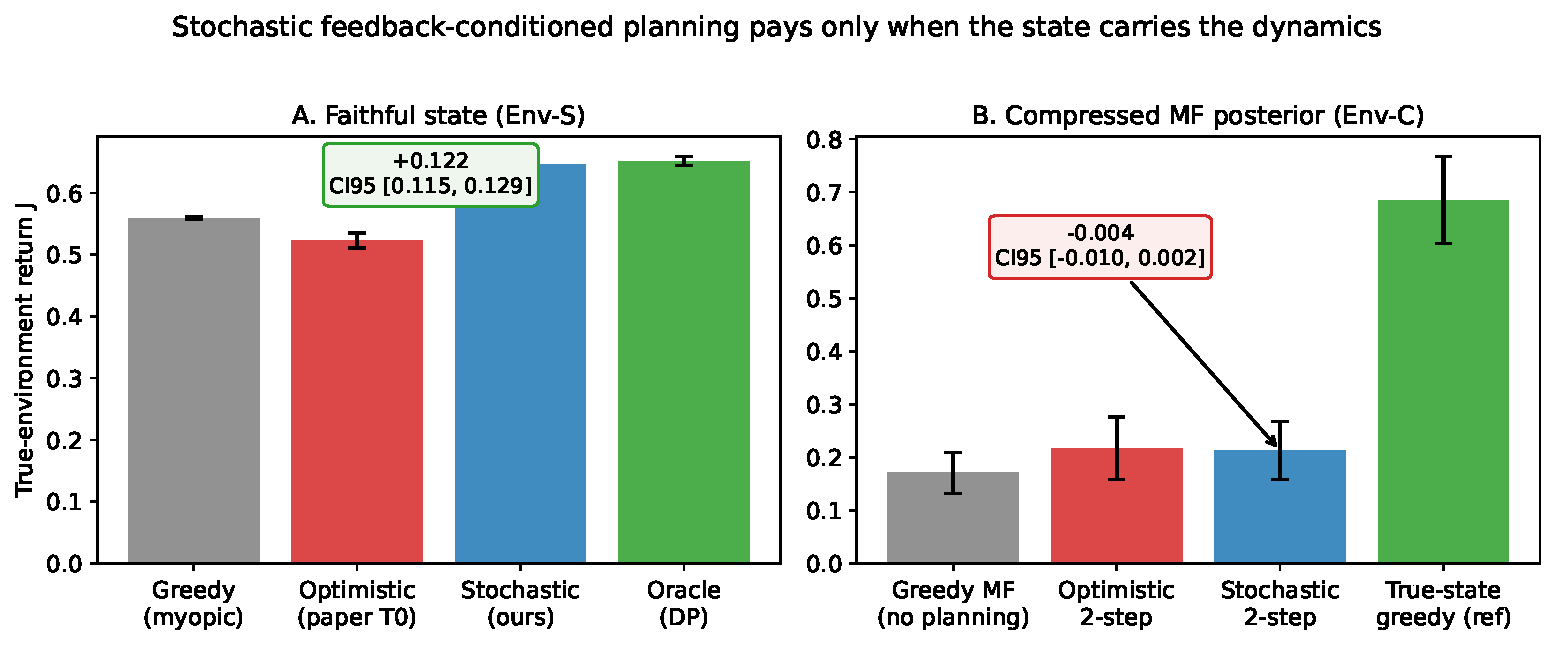
\includegraphics[width=\textwidth]{figures/main_figure.pdf}
\caption{The project's main message: stochastic feedback-conditioned planning pays only
when the state carries the dynamics. Left (faithful state, Env-S): stochastic $\approx$
oracle, $+0.122$ over optimistic. Right (compressed MF posterior, Env-C): no difference.}
\label{fig:main}
\end{figure}

\section{Limitations}

Env-S and Env-C are handcrafted; their contrast indicates the role of the state
representation but is not a strict single-variable isolation. Simulator results are
diagnostics, not evidence of real-user improvement. MovieLens-1M lacks exposure labels;
KuaiRand propensities are not verified, so no off-policy evaluation claims are made.
$V_{\text{logging}}$ (logging-policy value) is never $V^{\pi}$; target-policy value
remains unimplemented. The KuaiRand response model uses basic features; the $3.4$GB
statistic feature file is unused.

\section{Conclusion}

The answer to our research question is conditional: \textbf{learning stochastic user
dynamics makes model-based planning better than optimistic or greedy recommendation if
and only if the state representation carries the dynamics.} When the state is faithful,
a learned response model plus exact feedback-conditioned transitions recovers the
oracle; when the state is a compressed MF posterior, the transition model's
sophistication is irrelevant. This shifts the design question from ``how to plan
deeper'' to ``what state to build''. All results are reproducible with
\texttt{python run\_experiment.py}; the experiment log records every run with metrics.

\bibliographystyle{plain}
\bibliography{paper/references}

\end{document}
